%%% ======= Beamer ======
\documentclass[usenames,dvipsnames,t]{beamer}
% \documentclass[usenames,dvipsnames, handout]{beamer}
\beamertemplatenavigationsymbolsempty % remove toolbar at the bottom of slides
% \usepackage{appendixnumberbeamer} % for appendix
\usetheme{Madrid}
\usecolortheme{default}
\useinnertheme{circles}
\newcommand{\mtov}{M_{\text{TOV}}}

\usepackage{fontawesome}

% Define commands for social media icons with links
\newcommand{\twitter}{\href{https://twitter.com/ThibeauWouters}{\textcolor{black}{\faTwitter}}}
\newcommand{\linkedin}{\href{https://www.linkedin.com/in/ThibeauWouters}{\textcolor{black}{\faLinkedin}}}
\newcommand{\github}{\href{https://github.com/ThibeauWouters}{\textcolor{black}{\faGithub}}}

\setbeamercolor{author in head/foot}{bg=blue!10, fg=blue}
\setbeamercolor{title in head/foot}{bg=blue!10, fg=blue}
\setbeamercolor{date in head/foot}{bg=blue!10, fg=blue}

\makeatletter
\setbeamertemplate{footline}{
  \leavevmode%
  \hbox{%
  \begin{beamercolorbox}[wd=.333333\paperwidth,ht=2.25ex,dp=1ex,center]{author in head/foot}%
    \usebeamerfont{author in head/foot}\insertshortauthor\expandafter\ifblank\expandafter{\beamer@shortinstitute}{}{~~(\insertshortinstitute)}
  \end{beamercolorbox}%
  \begin{beamercolorbox}[wd=.333333\paperwidth,ht=2.25ex,dp=1ex,center]{title in head/foot}%
    \usebeamerfont{title in head/foot}\insertshorttitle
  \end{beamercolorbox}%
  \begin{beamercolorbox}[wd=.333333\paperwidth,ht=2.25ex,dp=1ex,right]{date in head/foot}%
    \usebeamerfont{date in head/foot}\insertshortdate{}\hspace*{2em}
    \insertframenumber{}%
%     / \inserttotalframenumber
    \hspace*{2ex} 
  \end{beamercolorbox}}%
  \vskip0pt%
}
\makeatother

\colorlet{beamer@blendedblue}{blue!70} % change color theme

\usepackage[style=numeric-comp,sorting=none,backend=biber]{biblatex}%<- specify style
\addbibresource{references.bib}%<- specify bib file

\usepackage{svg}


% For appendix
\newcommand{\backupbegin}{
   \newcounter{framenumberappendix}
   \setcounter{framenumberappendix}{\value{framenumber}}
}
\newcommand{\backupend}{
   \addtocounter{framenumberappendix}{-\value{framenumber}}
   \addtocounter{framenumber}{\value{framenumberappendix}} 
}

\setbeamertemplate{bibliography item}{\insertbiblabel} % improved references



% Other preamble stuff:
\usepackage{preamble}

%%% Uncomment for another color palette
% \definecolor{Logo1}{rgb}{0.0, 0, 0.7}
% \definecolor{Logo2}{rgb}{2.55, 2.55, 2.55}

% \setbeamercolor*{palette primary}{bg=Logo1, fg=white}
% \setbeamercolor*{palette secondary}{bg=Logo2, fg=white}
% \setbeamercolor*{palette tertiary}{bg=white, fg=Logo1}
% \setbeamercolor*{palette quaternary}{bg=white,fg=white}
% \setbeamercolor{structure}{fg=Logo1} % itemize, enumerate, etc
% \setbeamercolor{section in toc}{fg=Logo1} % TOC sections

% For figures
\usepackage{import}
\usepackage{xifthen}
\usepackage{pdfpages}
\usepackage{transparent}
\usepackage{mdframed}
\usepackage{subcaption}

\setbeamertemplate{caption}[numbered]


% --- Inkscape figures:
\newcommand{\incfig}[2][0.75\textwidth]{%
    \def\svgwidth{\columnwidth}
    \resizebox{#1}{!}{\import{Inkscape figs/}{#2.pdf_tex}}
}

% --- Height of frame
\newlength{\myheight}
\setlength{\myheight}{7cm}

\newlength\myheightfigureintext
\newlength\mydepthfigureintext
\settototalheight\myheightfigureintext{Xygp}
\settodepth\mydepthfigureintext{Xygp}
\setlength\fboxsep{0pt}


%------------------------------------------------------------
%This block of code defines the information to appear in the
%Title page
\title[Predict and prejudice] %optional
{Predict and Prejudice:\\ Classification of compact objects and model comparison using EOS knowledge}

\author[Thibeau Wouters]{Hauke Koehn, \textbf{Thibeau Wouters}, Henrik Rose, Peter T. H. Pang, Rahul Somasundaram, Ingo Tews, and Tim Dietrich \\ \vspace{2mm} \href{mailto:t.r.i.wouters@uu.nl}{t.r.i.wouters@uu.nl} \\ \vspace{2mm} \github \quad \linkedin \quad \twitter}

% \raisebox{-\mydepthfigureintext}{\fbox{
\includegraphics[height=\myheightfigureintext]{Figures/arxiv_logo_red_no_background.png}}}

\date[17/06/2024]{Extreme Matter call 17/06/2024}


%End of title page configuration block
%------------------------------------------------------------



%------------------------------------------------------------
%The next block of commands puts the table of contents at the 
%beginning of each section and highlights the current section:

% \AtBeginSection[]
% {
%   \begin{frame}[plain, noframenumbering]
%     \frametitle{Table of Contents}
%     \tableofcontents[currentsection]
%   \end{frame}
% }


%------------------------------------------------------------


\begin{document}

{

\usebackgroundtemplate{\transparent{0.15}{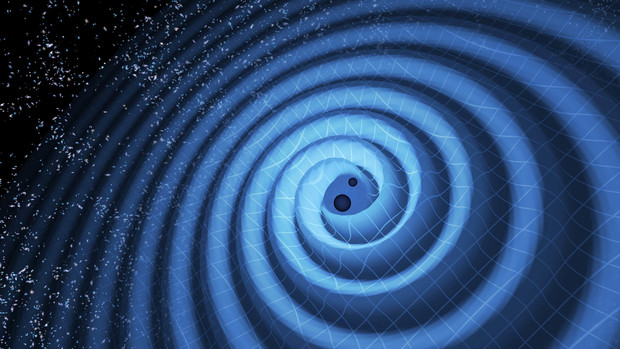
\includegraphics[width=\paperwidth,height=\paperheight]{Figures/GW-2.jpeg}}}

\begin{frame}[plain]
\titlepage

\begin{columns}
  \column{0.35\textwidth}
  \begin{figure}
    \centering
    \vspace{1.5mm}
    
\includegraphics[width=0.55\linewidth]{Figures/utrecht-university.png}
  \end{figure}
  \column{0.35\textwidth}
  \begin{figure}
    \centering
    
\includegraphics[width=0.55\linewidth]{Figures/Nikhef_logo-transparent.png}
  \end{figure}
\end{columns}

\end{frame}
}

% %The next statement creates the title page.
% \frame[plain]{\titlepage



% }


%---------------------------------------------------------
%This block of code is for the table of contents after
%the title page
% \begin{frame}[plain, noframenumbering]
% \frametitle{Table of Contents}
% \tableofcontents
% \end{frame}
%---------------------------------------------------------


\section{Introduction}

\begin{frame}{Overview}

  \def\x{4mm}
  \def\y{3mm}

  Our paper has several parts:
  \begin{itemize}
    \vspace{\x}
    \item Adding new NICER observation of PSR J0437-4715 (TBA)

    \vspace{\x}

    \item Classification of recent lower mass gap objects:
    \begin{itemize}
      \vspace{\y}
      \item  PSR J0514-4002E companion

      \vspace{\y}

      \item GW230529 primary~\cite{LIGOScientific:2024elc} (\textbf{this presentation})
    \end{itemize}

    \vspace{\x}
    
    \item Model selection: 
    \begin{itemize}
      \vspace{\y}
      \item  Comparison of NICER results for PSR J0030+0451

      \vspace{\y}

      \item Comparison of symmetry energy measurements
    \end{itemize}
    
  \end{itemize}
  
\end{frame}

\begin{frame}{Introduction -- GW230529}

  \begin{figure}
    \centering
    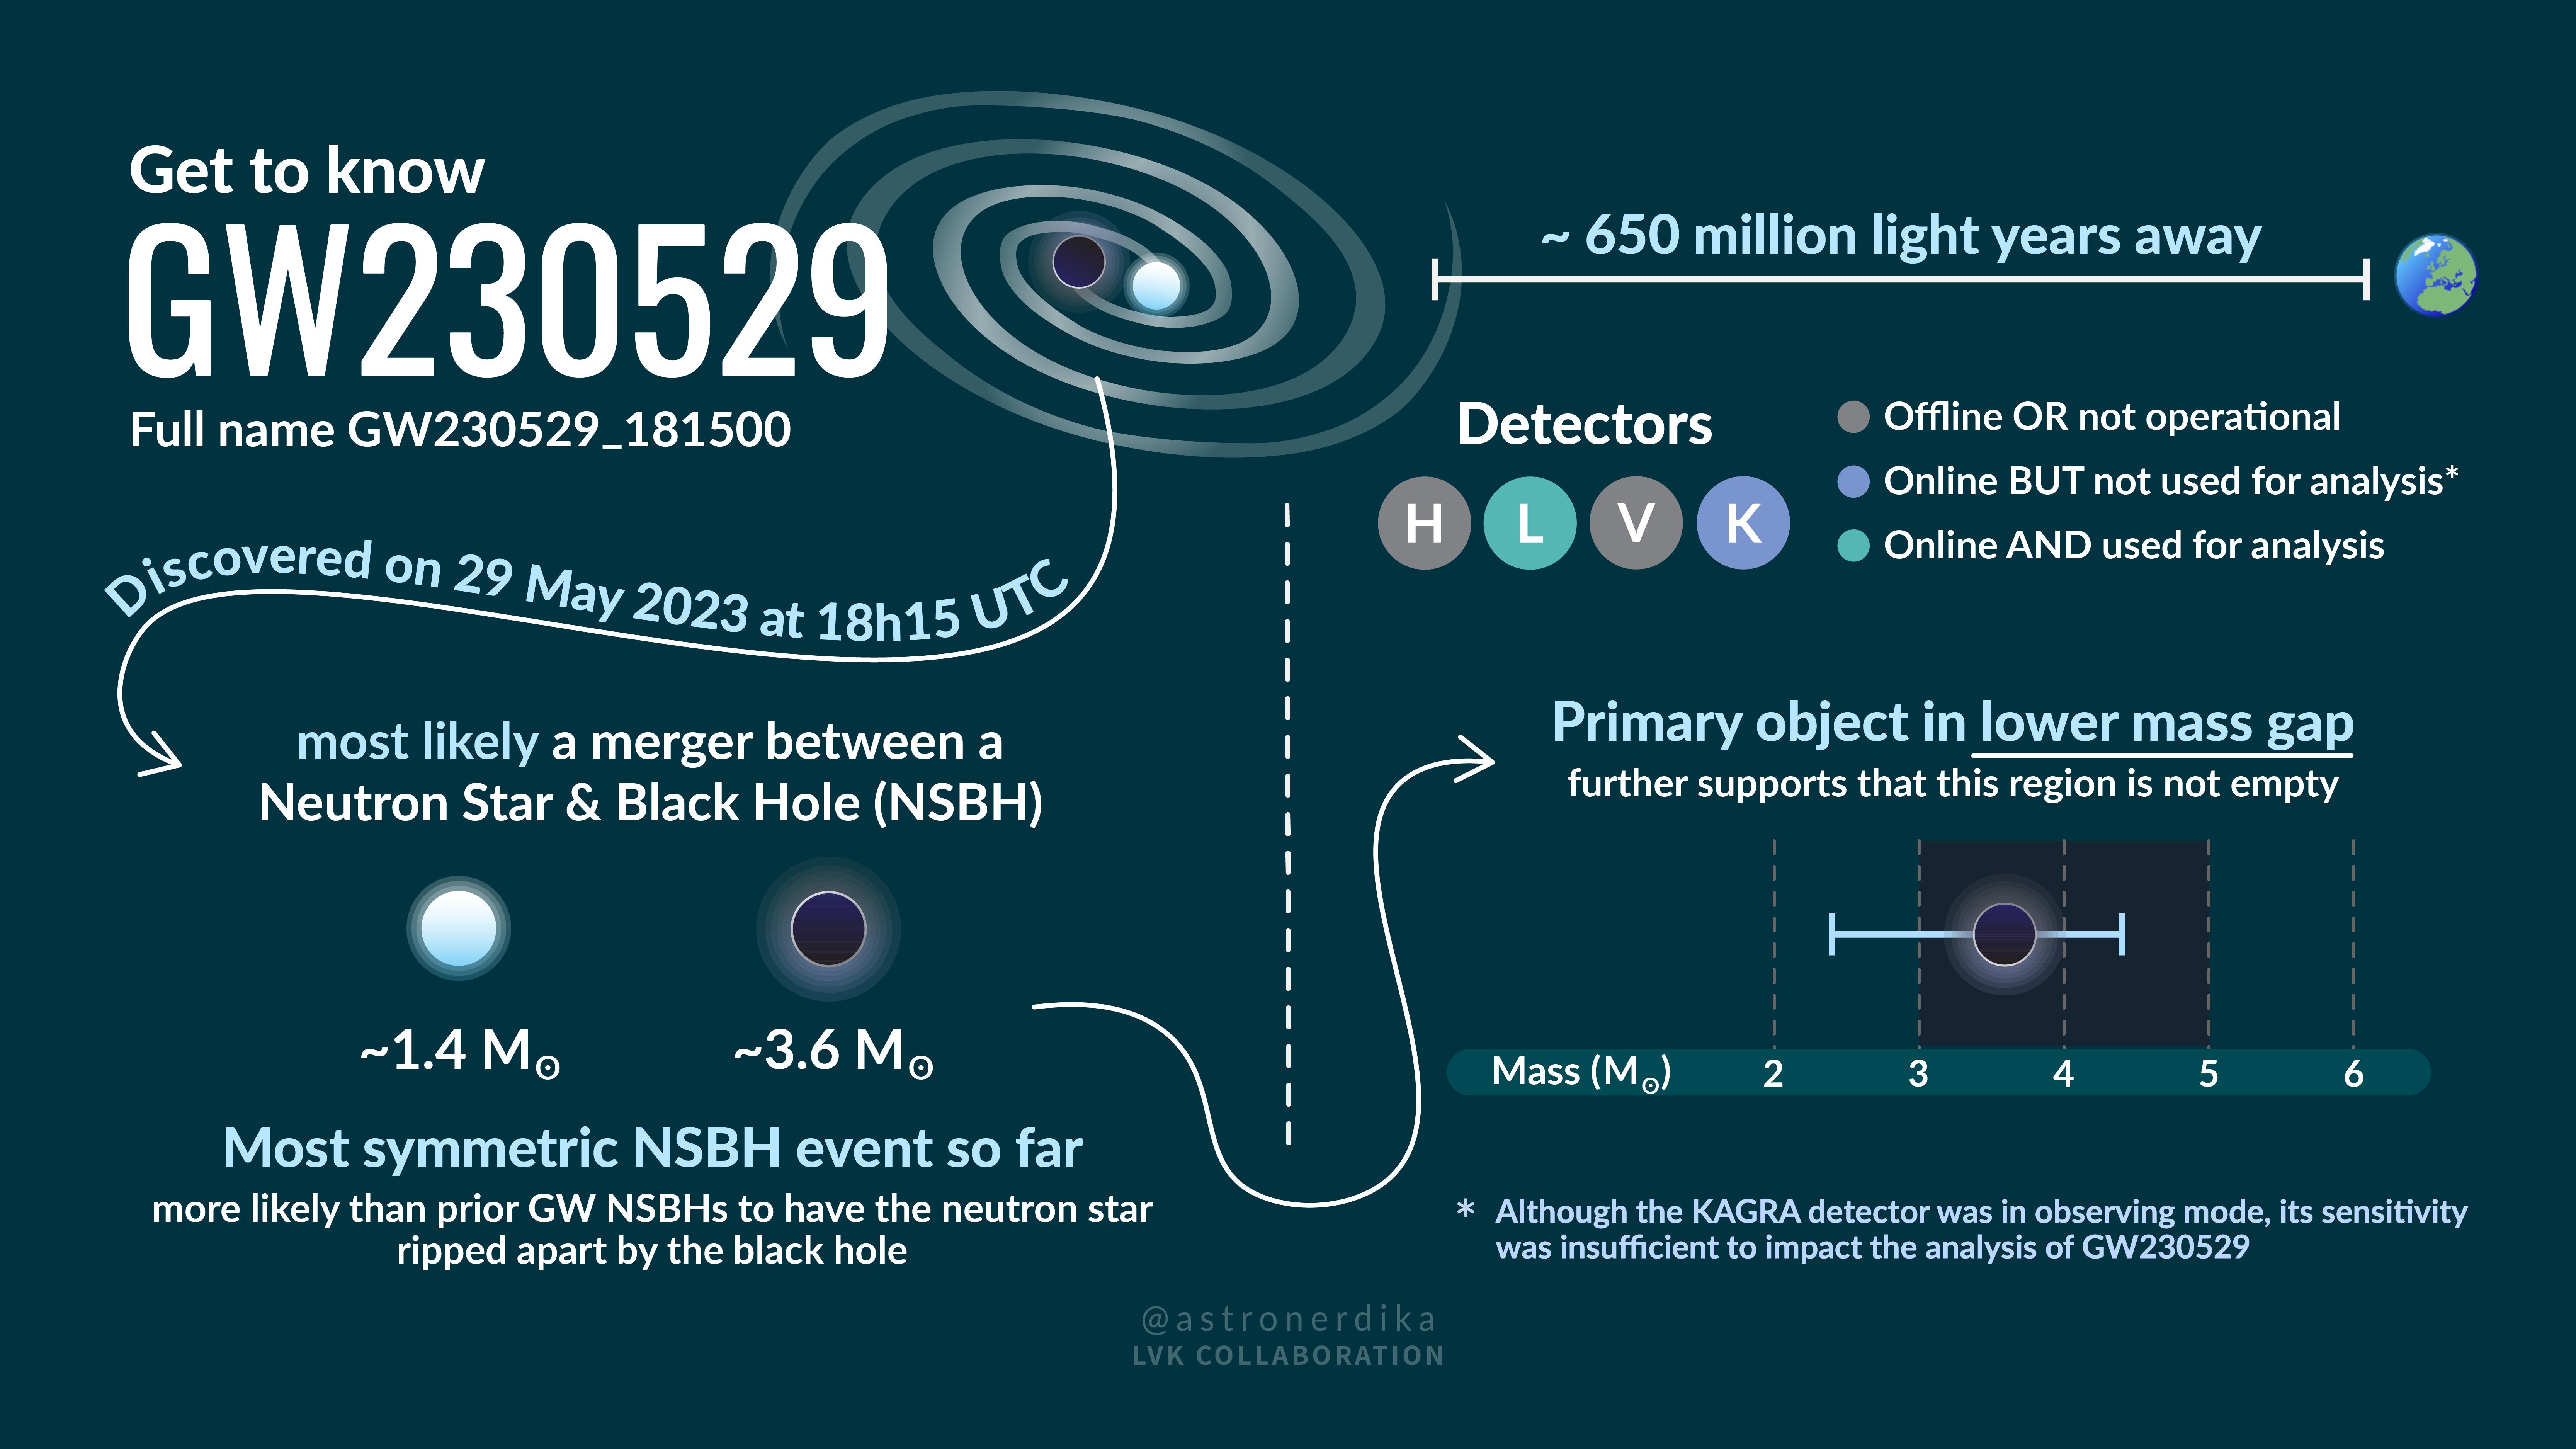
\includegraphics[width=1\linewidth]{Figures/GetToKnowGW230529_English.png}
  \end{figure}

  \scriptsize Credit: Shanika Galaudage \normalsize
\end{frame}
    
\begin{frame}{Equation of state constraints with \textsc{NMMA}}

\def\x{2mm}
\def\y{2mm}
\def\z{-2mm}

\vspace{\z}

\begin{columns}
  \column{0.9\textwidth}

  \textsc{NMMA} compiled sets of EOS constraints~\cite{Koehn:2024set}:
  \footnotesize
  \begin{itemize}

    \item Nuclear theory and experiments
    \item Radio observations pulsars, NICER, bursters, X-ray binaries
    \item GW170817 $+$ EM counterparts \& postmerger remnant

  \end{itemize}
  \normalsize

  \column{0.1\textwidth}

  \begin{figure}[t]
    \centering
    
\includegraphics[width=\linewidth]{Figures/NMMA logo.jpg}
  \end{figure}

  \vspace{-3mm}
  \small \textsc{NMMA} \normalsize
  
\end{columns}

\vspace{\x}
\begin{figure}
  \centering
  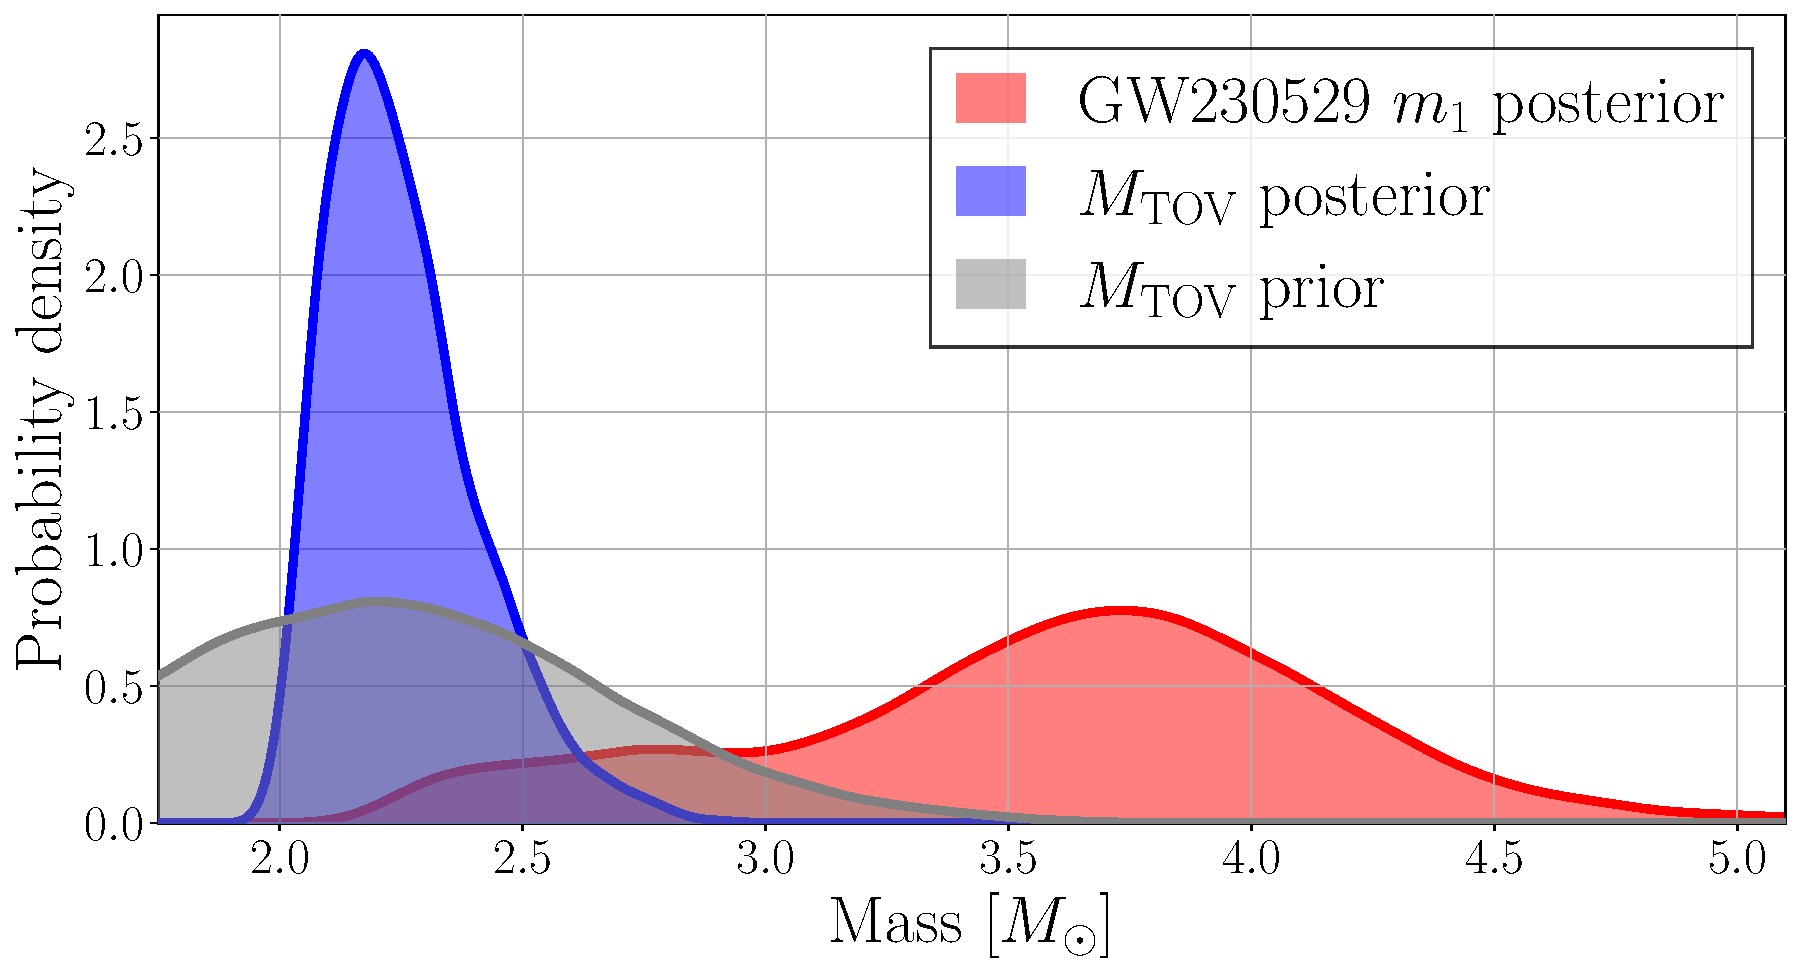
\includegraphics[width=0.7\linewidth]{Figures/mtov_gw230529_set_L1.pdf}
\end{figure}
\end{frame}


\begin{frame}{Methods -- EOS constraint sets}

  \small
\begin{table}[t]
  \renewcommand{\arraystretch}{1.1}
  \caption{Overview on the constraints contained within the three different constraint sets.}
  \label{tab:sets}
  \begin{tabular}{ l l p{7cm}}
  \toprule
  \toprule
  Set & Label & Description \\
  \midrule
  High confidence & 1 & Chiral EFT, pQCD, heavy radio pulsars, NICER \mbox{J0740+6620}, NICER \mbox{J0030+0451}, (NICER \mbox{J0437-4715}), GW170817\\
  \midrule
  More vigorous & 2 & Set 1, Black Widow \mbox{J0952-0607}, heavy ion-collisions, qLMXBs, GW170817+KN+GRB afterglow, CREX, PREX-II, Burster \mbox{4U 1702-429}, Burster \mbox{J1808.8-3658}, GW170817 postmerger\\
  \midrule
  Aggressive & 3 & Same as set 2, but for the remnant of GW170817 a hypermassive neutron star above the Kepler limit is assumed \\
  \bottomrule
  \end{tabular}
\end{table} 
\normalsize

\end{frame}

\begin{frame}{Methods -- Classification of compact objects}
  
  \def\x{3mm}

  \textsc{NMMA} \blue{sets of constraints $\mathcal{D}$} give posterior on $\mtov$. 
  
  Compare this against \red{GW230529}'s properties:

  \begin{itemize}
    \vspace{\x}

    \item Probability of primary being a neutron star: $P(NS)$:
    
    \begin{equation*}
      P(\text{NS}) = \!\int \!\differential\mtov \!\int_{0}^{\mtov}\! \! \! \differential \red{m_1} \ P(\mtov|\blue{\mathcal{D}}) P(\red{m_1}).
    \end{equation*}

    \vspace{\x}

    \item Spinning neutron stars can have higher masses: $M_{\rm{max}}(\rm{EOS}, \red{\chi_1})$:
    
    \begin{equation*}
      P(\text{NS}) = \int \differential M_{\rm{max}}\int_{0}^{M_{\rm{max}}} \! \! \!\differential \red{m_1} \int_0^1 \differential \red{\chi_1} \ P(M_{\rm{max}}|\blue{\mathcal{D}}, \red{\chi_1}) P(\red{m_1}, \red{\chi_1}) \, .
    \end{equation*}

    \vspace{\x}

    \item Use universal relation from Breu and Rezzolla for $M_{\rm{max}}$~\cite{Breu:2016ufb}
  \end{itemize}

\end{frame}


\begin{frame}{Classification results for GW230529 primary}

  \def\x{2mm}

  \begin{itemize}
    \vspace{\x}
    \item Set 1 and without spin agree well with LVK results~\cite{LIGOScientific:2024elc}. 

    \vspace{\x}

    \item Spin $+$ \textsc{PDB} raise $P(NS)$ to $\sim 17\%$.

    \vspace{\x}

    \item Set 3 (``aggressive'') drastically reduces $P(NS)$.
  \end{itemize}

  \begin{figure}
    \centering
    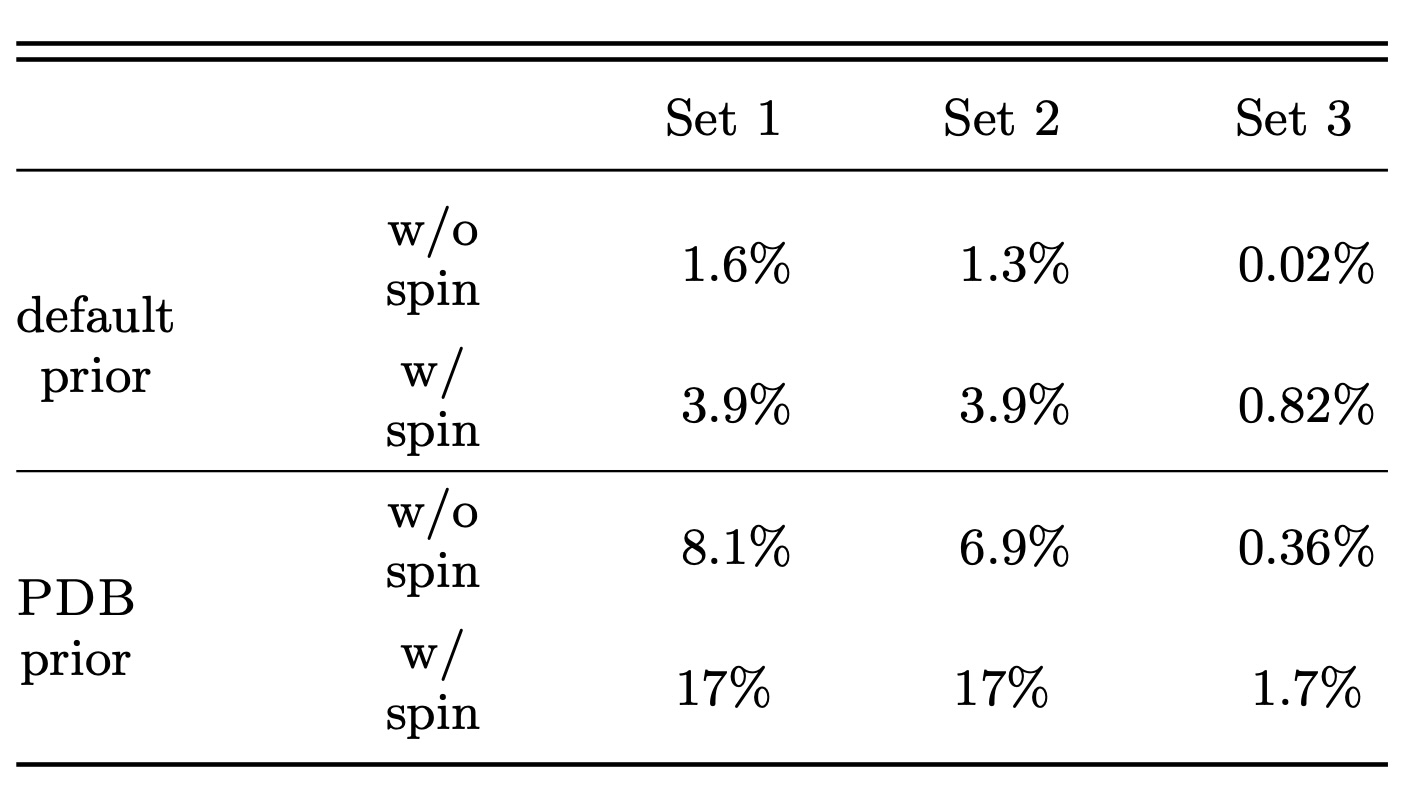
\includegraphics[width=0.7\linewidth]{Figures/extreme_matter_P_ns_table.jpg}
  \end{figure}
  \footnotesize
  \begin{center} 
    (\textsc{PDB}: Powerlaw + Dip + Break population model) 
  \end{center}
  \normalsize


\end{frame}


\section{Conclusion}

\begin{frame}{Conclusion}

  \def\x{10mm}

  \begin{itemize}
    \item GW230529: primary component in the lower mass gap

    \vspace{\x}

    \item \textsc{NMMA} has compiled current EOS constraints into 3 sets

    \vspace{\x}

    \item Accounting for spin raises $P(NS)$ for GW230529 primary to $\sim 17\%$ with \textsc{PDB}. The ``aggressive'' constraints gives $P(NS) \lesssim 1.7\%$

    \vspace{\x}

    \item Results are still consistent with black hole interpretation of GW230529 primary
  \end{itemize}
  
\end{frame}

\begin{frame}{References}

% \nocite{*}
\printbibliography
    
\end{frame}

% ======== APPENDIX  ==========

\appendix

\begin{frame}
\vfill
\centering
\textbf{APPENDIX}
\vfill
\end{frame}


\begin{frame}{Population informed posterior}

  Posterior obtained with \textsc{PDB} prior:
  \begin{figure}
    \centering
    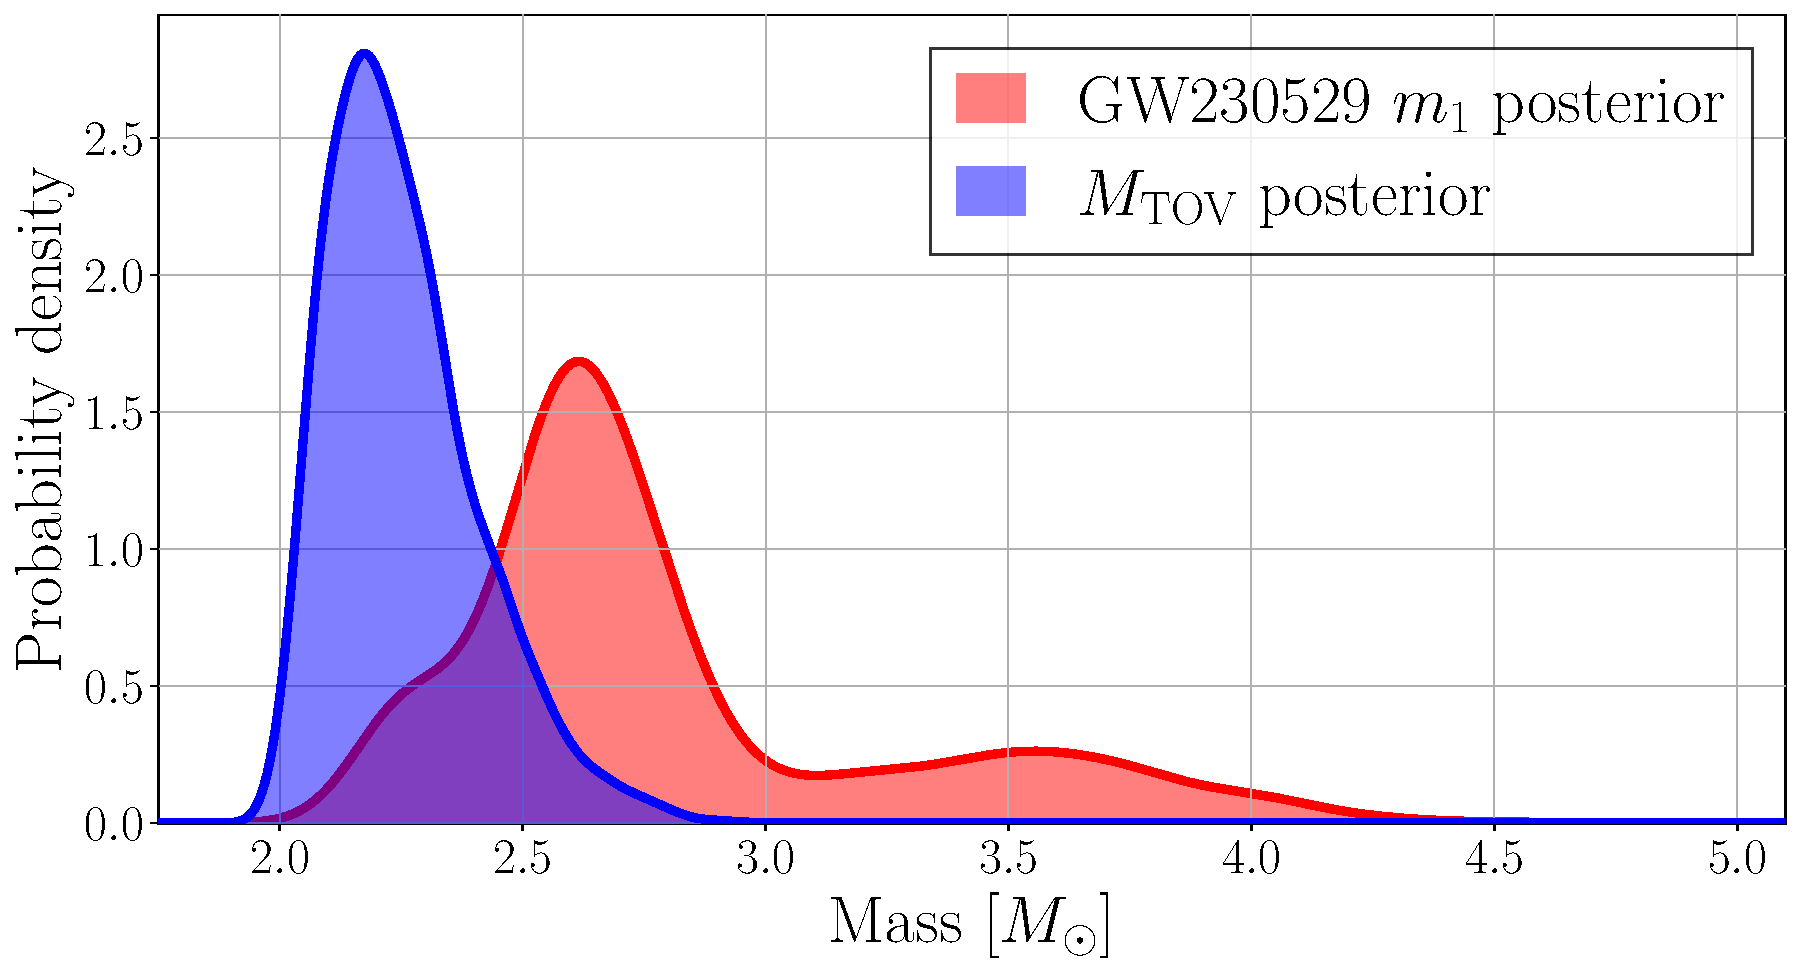
\includegraphics[width=0.9\linewidth]{Figures/mtov_gw230529_set_L1_pdb.pdf}
  \end{figure}    

\end{frame}

\begin{frame}{TOV mass posterior with set 3 (``Aggressive'')}

  \begin{figure}
    \centering
    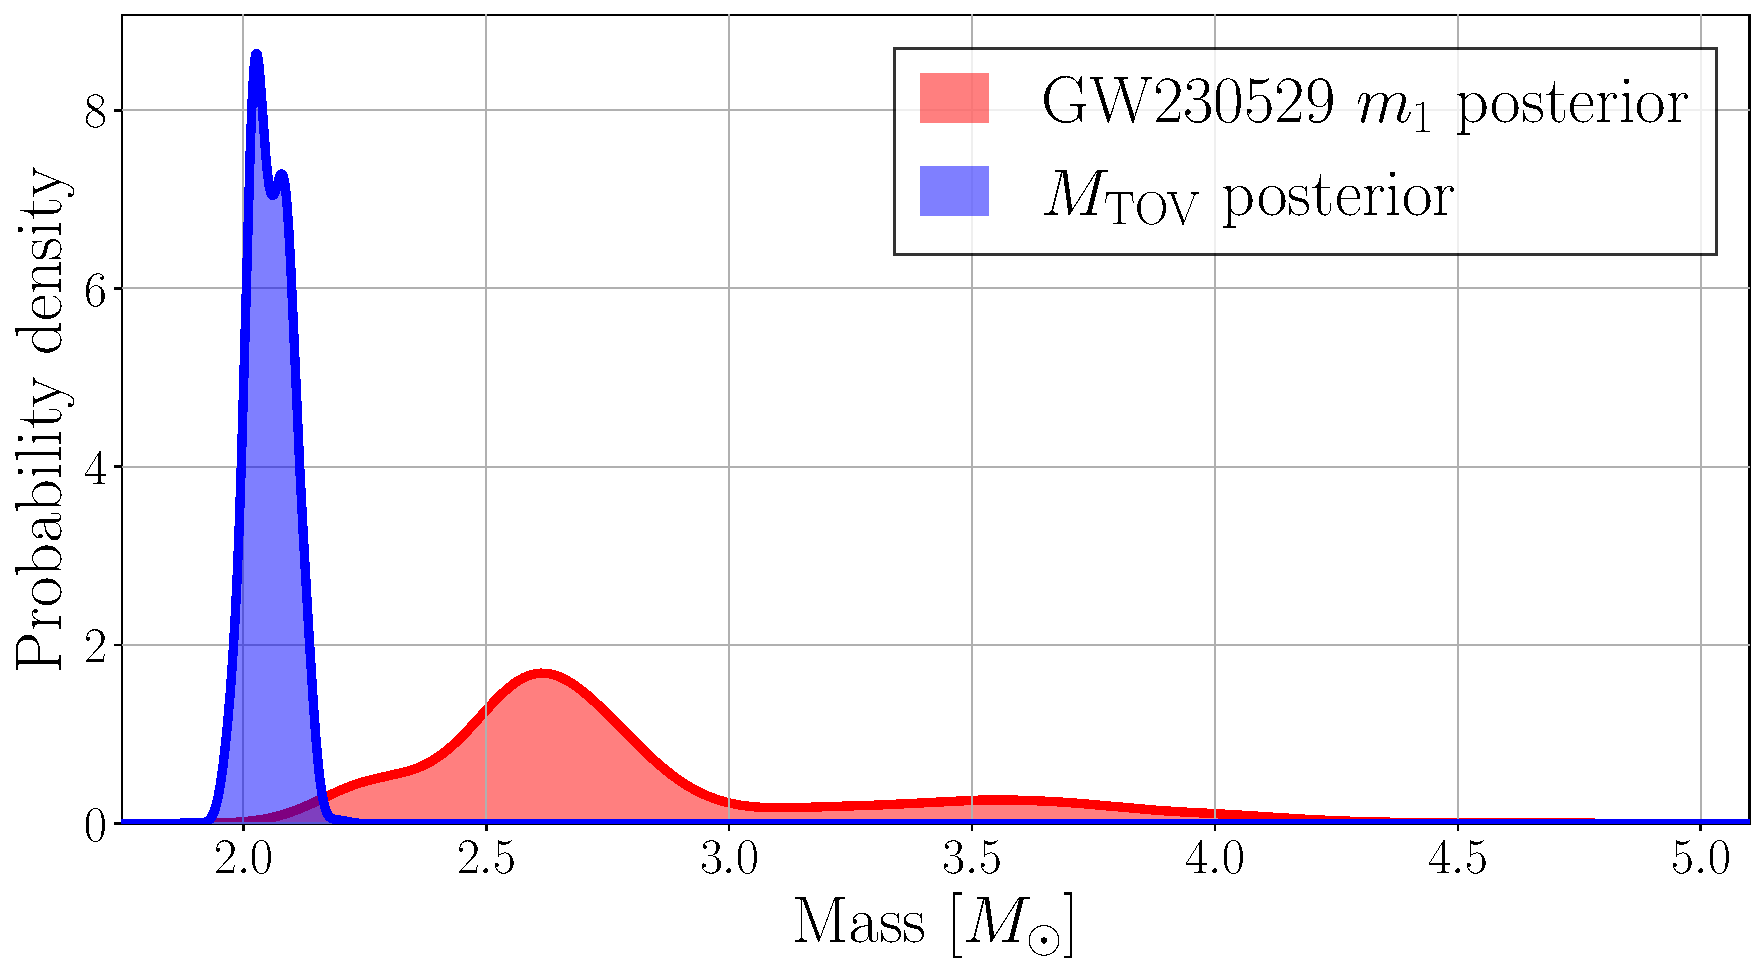
\includegraphics[width=0.75\linewidth]{Figures/mtov_gw230529_set_L3_pdb.pdf}
  \end{figure}

\end{frame}

% \begin{frame}{All probabilities for GW230529 primary being a NS}

%   \small
%   \begin{table}
%     \renewcommand{\arraystretch}{1.25}
%     \centering
%     % \caption{Probability that the primary component of GW230529 is a \ac{NS} when considering the posterior samples inferred when using the default priors (explained in the main text) and the priors informed by the \textsc{Power law + Dip + Break} (\textsc{PDB}) population model.}
%     \label{tab: classification results GW230529}
%     \begin{tabular*}{0.975\linewidth}{@{\extracolsep{\fill}} l c c | c c c}
% \toprule\toprule
%   & & spin & $1$ & $2$ & $3$ \\
% \midrule
% \multirow{4}{*}{GW230529} & \multirow{2}{*}{default} & $\cross$ & $\phantom{0}1.63\%$ & $\phantom{0}1.37\%$ & $\phantom{0}0.02\%$ \\ 
% & & \checkmark & $\phantom{0}3.96\%$ & $\phantom{0}3.97\%$ & $\phantom{0}0.82\%$  \\ \cline{2-6}
% & \multirow{2}{*}{\textsc{PDB}} & $\cross$ & $\phantom{0}8.26\%$ & $\phantom{0}6.98\%$ & $\phantom{0}0.38\%$ \\ 
% & & \checkmark & $17.96\%$ & $17.83\%$ & $\phantom{0}1.79\%$ \\ 

% \bottomrule
% \end{tabular*}
% \end{table}
% \normalsize
% \end{frame}


\end{document}